% !TEX root = ../main.tex
\clearpage
\section{产品设计与使用流程}
\subsection*{以研究问题为中心的投研工作台}\label{page:09}
\noindent\textbf{低空智研的产品形态是一张面向事件驱动研究的工作台，而不是一张只给出推荐顺序的看板。}研究者从一个已登记事件出发，在同一研究现场依次阅读事件事实、产业传导路径、公司比较、评分构成、证据摘录和运行来源。界面将这些对象放在一份报告上下文中，是为了让使用者能够沿结论反向检查：某家公司为何出现在研究队列中、该公司受到何种方向的影响、系统依据了哪条路径、引用来自何处。

\begin{center}
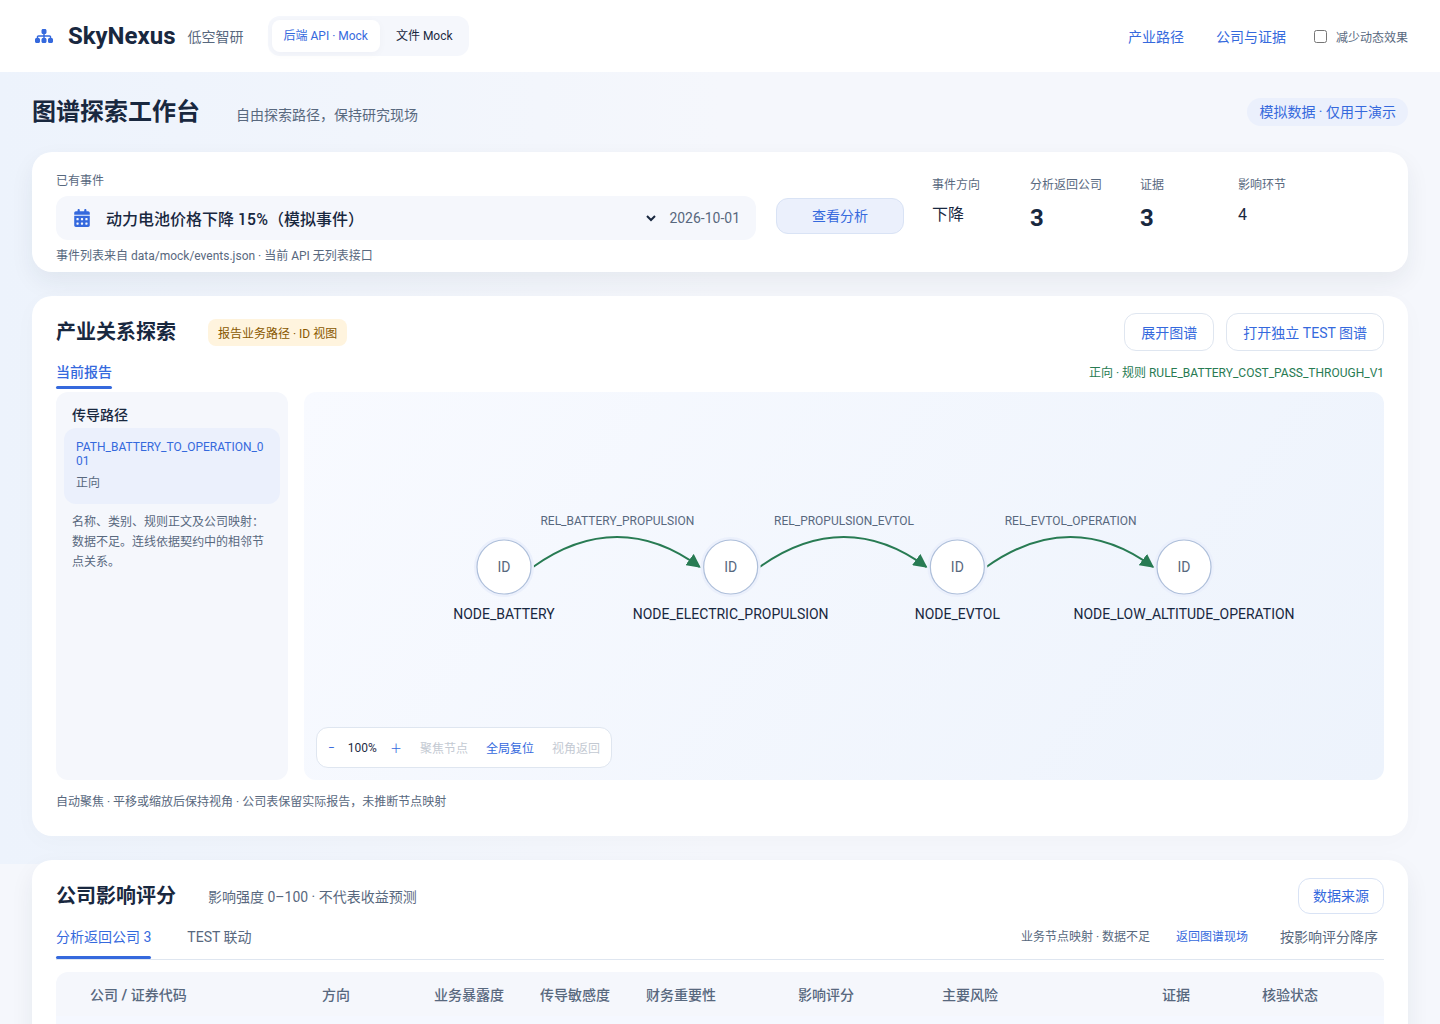
\includegraphics[width=0.94\linewidth,height=0.43\textheight,keepaspectratio]{assets/hongyulyu714-prog/fig-workbench.png}
\PlanFigureCaption{图9-1}{当前业务工作台截图。页面在“后端API·Mock”模式下展示已选事件、业务图谱、公司影响、证据抽屉和研究现场；截图来源于仓库\texttt{docs/screenshots/03-business-1440.png}，采集清单记录的实现提交为\texttt{86a440a}。}
\end{center}

图9-1所示界面把“得到答案”改造成“完成研究动作”。研究者先确认事件与版本，再主动提交分析；返回报告后，先阅读图谱中的有序业务ID，再查看与路径相关的公司卡片；当公司分数或传导解释需要确认时，可以打开证据抽屉并回到来源与运行信息。整个过程不是以页面排序替代判断，而是为研究者提供一份具备对象层次的证据索引\cite{lhy-frontend,lhy-architecture}。

\begin{center}\small 表9-1\quad 工作台的研究动作、输出对象与使用价值\par\vspace{1mm}
\begin{tabularx}{\linewidth}{p{0.20\linewidth}p{0.30\linewidth}X}
\toprule
研究动作 & 页面输出对象 & 对投研工作的价值\\
\midrule
选择并确认事件 & 事件名称、\texttt{event\_id}、来源、方向、版本与状态 & 将研究对象固定在明确的时间和来源口径内，避免不同模块围绕相似文本分别理解。\\
发起一次分析 & 报告ID、\texttt{run\_id}、生成时间、数据版本和异常状态 & 让每次研究请求成为可重放的记录，而非一次性的页面刷新。\\
阅读产业路径 & 节点ID、关系ID、方向、规则入口和路径证据 & 将“产业相关”展开为一系列可逐边核验的传导命题。\\
比较公司影响 & 证券代码、角色、方向、影响分、风险标记和证据ID & 把公司筛选从概念罗列推进为可审阅的候选研究队列。\\
打开证据与来源 & 标题、日期、摘录、URL、可信度、核验状态与运行信息 & 支持研究者回到原始材料，检验结论是否超出证据的支持范围。\\
\bottomrule
\end{tabularx}\end{center}
\SourceNote{当前前端能力、模式与截图口径来自\texttt{docs/FRONTEND\_DEMO.md}及其截图清单；访问日期：2026-10-15。}

产品设计的重点在于保持研究链的连续性。事件、路径、公司、评分和证据在数据层上分别管理，在阅读层上却被组织为一条可追溯的论证链；这既减少了研究者跨文件寻找依据的成本，也使后续替换数据源时可以准确识别报告中的变化来自事件、图谱、财务还是证据层。当前工作台使用已登记的Mock事件验证这一交互闭环，随后将承接通过审核的数据版本和真实事件级评测。
